\documentclass[11pt]{article}
\usepackage[preprint]{acl}
\usepackage{times,latexsym}
\usepackage[T1]{fontenc}
\usepackage[utf8]{inputenc}
\usepackage{microtype,graphicx,booktabs,amsmath}
\title{Examples, Persistent Rules, and Information Limits in Agent Annotation}
\author{Research Working Draft\\Authors to be confirmed}
\begin{document}
\maketitle
\begin{abstract}
Annotation manuals combine general definitions with examples, exceptions, and domain conventions. We investigate whether fixed-weight agents benefit from converting a small purchased example set into persistent rules, beyond retaining access to the original examples. Our protocol compares retrieval, free-form notes, and an error-guided rule-addendum comparator across linguistic supersense annotation and political-topic coding. Nested additional-example budgets separate supervision from adaptation compute, while frozen evaluation assets prevent test feedback. An audit of the political dataset also identifies an information limitation: exactly identical summaries can have different published labels. This is distinct from failure to learn a rule. We report real experiments and their operational status, including earlier API diagnostics that cannot support clean capability comparisons. The study measures additional deployment-time adaptation under public manuals and pretrained models; it does not establish from-scratch sample complexity, unrestricted agent self-evolution, or a universal sufficient number of examples.
\end{abstract}
\noindent\fbox{\parbox{0.94\columnwidth}{\textbf{Review draft.} Completed bounded experimental matrix; limitations still apply.}}


\section{Introduction}
A human annotator can read a definition yet remain uncertain about a particular construction. Examples may resolve an ambiguity that is dispersed across a manual, insufficiently explained, or dependent on domain knowledge. Occupational roles expressed through apposition in Uniform Meaning Representation motivated this question. We do not assume that the official UMR guideline lacks a relevant rule: that specific omission has not been expert-verified.

The useful empirical question is not whether machines can read guidelines at all. Guideline-conditioned extraction already exists \citep{gollie}, and iterative guideline refinement has been studied directly \citep{kim2026refining}. We instead ask when persistent rules help an agent beyond searchable access to the same examples, how behavior changes with additional supervision, and which apparent learning failures arise from missing information rather than inadequate adaptation.

We operationalize an agent as a fixed-weight model that repeatedly chooses authorized tools to inspect a long manual, retrieve purchased examples, and read or write persistent assets. This controlled interface is narrower than an unrestricted coding assistant. Earlier program-permission experiments produced no program executions; they cannot estimate an effect of executable self-modification. The present main comparison consequently concerns policy adaptation through persistent text.

Our design spans linguistic annotation and political-topic coding. Visual annotation is retained as a diagnostic case, not treated as equivalent evidence: the acquired Fashionpedia taxonomy is not a complete operational handbook. We distinguish deployment-time annotation budget, existing manual examples, model prior knowledge, and compute. None is silently counted as another.

\section{Related Work and Scope}
GoLLIE demonstrates guideline-conditioned information extraction \citep{gollie}; GuideBench evaluates domain-oriented guideline following \citep{guidebench}. These precedents rule out the claim that models can only learn from large labeled datasets and cannot use written instructions.

The closest study, \citet{kim2026refining}, predicts annotations on an adaptation set, groups errors, contrasts them with correct cases, derives principles with negative constraints, and rewrites the guideline. It retains improvements measured on the adaptation set and evaluates independently. Ten training documents per biomedical task provide refinement evidence; 100 development documents provide evaluation. Their work already covers persistent guideline refinement, limited supervision, independent evaluation, and model differences. It explicitly leaves varying supervision amounts to future work.

Our error-guided comparator adapts this workflow to rule addenda and a bounded update per budget. It is neither a faithful full-manual rewrite nor a numerical reproduction of their biomedical results. The proposed contribution is a matched-evidence comparison over nested budgets with cross-domain information audits. Whether the measured effects justify an ACL contribution remains subject to the results and limitations below; more datasets alone do not establish novelty.

\section{Benchmark Selection}
\subsection{SNACS}
SNACS distinguishes the scene role of an adposition from its lexical function. We use STREUSLE \citep{streusle}, pinned to commit \texttt{8ba61fe4}, and the complete SNACS v2.6 manual: 114 pages and 541 uniquely numbered example groups. A group may contain several contrasts or subexamples; it is not a count of independently labeled targets. Budget zero therefore means zero \emph{newly purchased} examples, not zero supervision.

The supplied-span projection retains text, tokens, and target locations while stripping syntactic and other semantic gold. Train/dev/test contain 1,911/267/259 sentences, 4,553/462/485 decisions, and 347/156/146 documents. The official 52-label ontology determines validity. We previously verified target denominators and three accuracy measures against the unmodified upstream scorer for 60 valid-output control configurations. This does not establish official equivalence for target identification or arbitrary invalid outputs.

The new agent test sample comprises 64 documents, 114 sentences, and 202 targets. It excludes all documents used in the earlier small API agent pilot. The corpus was already used for non-LLM controls; we do not describe it as wholly unseen by the research process. No held-out label is provided to the agent or used to update its assets.

\subsection{CAP Pennsylvania}
The Comparative Agendas Project publishes Pennsylvania bills and resolutions with a paired 73-page \emph{Policy Topics Codebook} \citep{cappa}. Unlike a label-name inventory, it contains decision rules, examples, and cross-topic exceptions: 194 printed \texttt{Rule:} sections and 240 explicit code headings. For example, general appropriations receive a specified fiscal code, while some industry-specific tax policies follow the substantive policy area rather than a general taxation category.

We predict the local \texttt{pa\_code} from the published \texttt{nuc} summary. The crosswalked \texttt{subtopic} is different in 26,411 records and is not a substitute target for the PA manual. The controller withholds all derived labels and filters, year, sponsor, chamber, and bill identifiers. Opaque IDs associate predictions with records. The source has 102,727 rows from 1979--2016, despite a filename ending in 2019. Seven observed codes do not match explicit handbook headings; their 17 rows are quarantined without guessed corrections. This leaves 102,710 rows and 231 observed supported codes.

To prevent repeated legislation leaking across splits, we first group lowercase, whitespace-normalized summaries. We then generate near-duplicate candidates with 64 MinHash values in 16 bands, verify five-word-shingle Jaccard similarity of at least .85, and take connected components. This merges 4,063 components over the full input. Candidate retrieval is approximate, overfull bands are skipped, and transitive endpoints need not exceed the pairwise threshold; we do not claim exhaustive near-duplicate removal. A fixed label-blind hash assigns entire families to a custom 70/15/15 split. Supported train/dev/test have 43,625/9,552/9,281 families; intersections are empty.

The test sample has 128 families and 215 records, covering 73 of the 240 valid handbook codes. Forty observed codes have only one test record. This is insufficient for robust per-class claims. Official documentation supports project construction by faculty-supervised students, not a claim that every row has independently verified human double annotation. The 2019 manual is officially paired with historical data; comprehensive relabeling to that manual version is unverified. Summary-only annotation is not proven equivalent to the original full-document workflow.

\subsection{Why Not Simply Add Manifesto and Fashionpedia?}
Manifesto is a relevant political coding candidate \citep{manifesto}, but the needed resource is its coded quasi-sentence Corpus, not aggregate party percentages. We obtained the 2021 and 2026 handbooks; legitimate sentence-level access still requires an account key or export. Segmentation, handbook version, country, election, translation, and wider document context would require control. Its handbook allows progressively broader context, including political background; restricting inputs to isolated sentences would change the task.

Fashionpedia \citep{fashionpedia} adds perception and domain knowledge as well as annotation policy. We acquired genuine images and official labels, using supplied regions to avoid conflating localization with classification. However, the available 46-category/294-attribute names and hierarchy are not a full annotation manual. The API demonstration taxonomy also differs from the final ontology. Thus our real-image pilot validates plumbing but does not identify a boundary of learning from complete guidelines. ContractNLI has suitable public document splits, but its example-oriented per-hypothesis guidelines were not found in the inspected public release; its hypothesis list alone is not a replacement handbook.

\section{Information Limits Before Model Evaluation}
Let $n(x,y)$ count records with exactly the same raw summary $x$ and published code $y$. A fixed-state classifier constrained to output the same label for the same text can match at most
\begin{equation}
 U=\frac{\sum_x\max_y n(x,y)}{\sum_{x,y}n(x,y)}
\end{equation}
of this fixed empirical dataset. This is a descriptive consistency bound, not a guarantee for new samples or a human ceiling.

After unsupported-code quarantine, there are 540 raw-exact conflict groups containing 2,066 records. At most 1,416 of these records can simultaneously match under the same-text/same-output restriction: 68.54\%. Across all 102,710 records, at least 650 cannot simultaneously match, giving 99.37\% overall. These counts use the original raw string, without normalizing away potentially useful distinctions. For example, ``An Act providing for broadcast employment contracts. occurs twice with broadcast-industry code 1707 and once with labor-relations code 504. The manual itself notes that industry-specific labor observations may follow their substantive industry; the repeated text alone does not establish which historical coding decision is correct. This is an audited disagreement, not expert adjudication or an invented test example.

The conflicts may reflect missing full-document context, policy changes, or noise; we have not adjudicated them into one cause. The actual agent sees opaque instance IDs and a batch of other unlabeled texts, so this bound is \emph{not} its hard accuracy ceiling. Different context or state also invalidates the same-input premise. Only three raw-conflict groups occur in the sampled test set, precluding a strong experimental ambiguity-subset claim. The full-source audit nevertheless demonstrates why increasing examples alone need not resolve every published-label inconsistency.

\section{Experimental Protocol}
\subsection{Evidence and Adaptation}
A trusted controller owns gold, the purchase ledger, and metrics. Agents inspect manual fragments through \texttt{read\_material} and lexical \texttt{search\_materials}; they retrieve purchased examples individually, in groups of up to 16, or by lexical search over public text. Test labels never enter tool results. A full manual is not injected into ordinary evaluation contexts.

Budgets are 0, 4, 16, and 64 purchased records with seeds 11, 23, and 47. For each seed, rows are shuffled and the first row from each distinct training family is retained. This produces nested sequences and avoids buying multiple rows from one family, but is not uniform family sampling: larger families are more likely to occur early. Models and conditions share the sequence. One SNACS record reveals all retained target pairs; one CAP record reveals one code. We report both records and decisions. All authorized examples are charged, whether or not an agent reads every one.

\paragraph{Frozen retrieval.} The system retains the original manual and every purchased example, with no writable persistent state.
\paragraph{Free notes.} A bounded adaptation episode may write reusable rules and exceptions. Evaluation retains access to original examples as well as frozen notes.
\paragraph{Error-guided moderation.} The controller probes purchased adaptation inputs, with no accessible labeled exemplars, under the full current guideline and assets. It selects the largest prediction--gold discrepancy group and correct contrasts, capped at five each. Three stages describe the error pattern, derive an IF/THEN principle with negative constraints, and update a policy addendum. A second adaptation probe accepts a changed addendum only upon strict accuracy improvement; otherwise the prior assets are restored. Failed or incomplete probes cannot generate a semantic error or justify acceptance. There is one proposal per budget, not unbounded optimization. Full-guideline probe context and additional update calls are method-specific compute, explicitly not compute-matched.

Training-set improvement is only an update rule; it may overfit and is not evidence of generalization. Budget-zero retrieval is a single shared starting point. It is not replicated into artificial independent adaptation trajectories.

\subsection{Models and Execution}
We use the official logged-in Codex CLI subscription channel with \texttt{gpt-6-sol} and \texttt{gpt-6-luna}, both at medium reasoning effort. These are mutable aliases, not immutable dated snapshots or a controlled parameter-count comparison. CLI version, model catalog, prompts, source hashes, token usage, latency, and actions are recorded. Native host features are disabled; actions use a strict output schema and are executed by the external controller. Unrecognized or forbidden native-tool events halt the backend. A synthetic sentinel probe did not reveal host-file contents. This audited interface is not proof that a read-only OS sandbox hides all host files.

Each actor call is ephemeral but receives the serialized episode history. The CLI's own system context contributes substantial tokens; the comparison concerns these complete CLI systems. Subscription tokens are not converted to invented API-dollar costs. The initial shared ceiling was 6,000 calls. An operational amendment raises it to 18,000 after observed search-call volume showed the initial estimate inadequate; this amendment follows some baseline test inference and is disclosed rather than called an untouched preregistration. A recorded policy-refused prompt is terminal and never resubmitted. Capacity interruptions receive bounded, delayed continuation on the same model with lower concurrency. Exact saved conversation history is resumed, and completed outcomes are never rerun to select favorable answers. Original and continuation settings and source hashes are retained.

\subsection{Held-Out Evaluation and Metrics}
Evaluation uses 16 fixed batches per task: four SNACS documents or eight CAP families per batch. Every condition receives the same batches and order, begins from immutable assets, and receives no prior-batch predictions. Within a batch, unlabeled examples can inform one another. We therefore describe batch-level inference, not independent instance resets. Prediction is capped at 12 actor calls, free adaptation at 24, and each moderation update stage at six. Full-context probes have two calls.

Primary outcomes are joint role/function accuracy for SNACS and record accuracy for CAP. We also retain output validity, completion, family-macro accuracy, label support, and macro-F1. CAP inventory macro-F1 includes all 240 handbook codes: on this sample even perfect predictions yield only $73/240=30.42\%$. Observed-label macro-F1 avoids interpreting absent-class zeros as inability on present classes, although rare-class estimates remain unstable.

Differences use paired descriptive resampling over adaptation seeds and evaluation batches. Three seeds and 16 batches limit interval calibration. We show every trajectory without monotonic smoothing and report observed threshold attainment at 70\%, 80\%, and 90\%; unreached thresholds do not license extrapolating a sufficient example count. Public pretraining exposure and guideline-native examples rule out a from-scratch sample-complexity interpretation.

\section{Results and Operational Accounting}
\begin{table*}[t]
\centering\small
\begin{tabular}{llrrrr}
\toprule
Task & Tier & $B$ & Retrieval & Notes & Moderation \\
\midrule
SNACS & Luna & 0 & 40.1 (1) & shared B0 & shared B0 \\
SNACS & Luna & 4 & 37.6 (1) & 41.1 (1) & 40.1 (1) \\
SNACS & Luna & 16 & 43.6 (1) & 43.1 (1) & pending \\
SNACS & Luna & 64 & 45.5 (1) & 49.0 (1) & pending \\
SNACS & Sol & 0 & 71.3 (1) & shared B0 & shared B0 \\
SNACS & Sol & 4 & 71.8 (1) & 69.8 (1) & 70.8 (1) \\
SNACS & Sol & 16 & 67.8 (1) & 75.2 (1) & 71.8 (1) \\
SNACS & Sol & 64 & 76.7 (1) & 76.2 (1) & pending \\
CAP PA & Luna & 0 & 44.7 (1) & shared B0 & shared B0 \\
CAP PA & Luna & 4 & 32.6 (1) & 38.6 (1) & pending \\
CAP PA & Luna & 16 & 35.8 (1) & 31.6 (1) & pending \\
CAP PA & Luna & 64 & 41.9 (1) & pending & pending \\
CAP PA & Sol & 0 & 64.2 (1) & shared B0 & shared B0 \\
CAP PA & Sol & 4 & 64.7 (1) & 58.6 (1) & 61.9 (1) \\
CAP PA & Sol & 16 & 61.9 (1) & 65.6 (1) & 69.3 (1) \\
CAP PA & Sol & 64 & 65.1 (1) & 66.5 (1) & pending \\
\bottomrule
\end{tabular}
\caption{Observed primary accuracy (\%) and number of completed adaptation trajectories in parentheses. Pending cells have no imputed score. B0 is one shared retrieval starting point. Comparisons with incomplete or unequal trajectory counts are provisional. All evaluated targets, including refusals and call exhaustion, remain in denominators.}
\label{tab:subscription}
\end{table*}
At this snapshot, 32 of 112 configuration cells are complete. The transport ledger records 4,701 actor requests. Completed cell scores appear in Table~\ref{tab:subscription}; missing cells are not scored as zero. Operational statuses are retained separately from semantic errors.
No full three-seed paired condition contrast has completed in this snapshot; no adaptation-effect estimate is claimed.
\paragraph{Matched non-LLM controls.} All 45 control cells completed on the same new study samples and purchased trajectories. At $B=64$, mean primary accuracies over the three seeds are: snacs majority 13.4\%; snacs lexical majority 24.8\%; snacs tfidf nearest 15.7\%; cap pa majority 3.3\%; cap pa tfidf nearest 13.2\%. These controls do not receive guideline knowledge. They are diagnostics, not substitutes for a strong full-context model baseline.
\begin{figure*}[t]
\centering
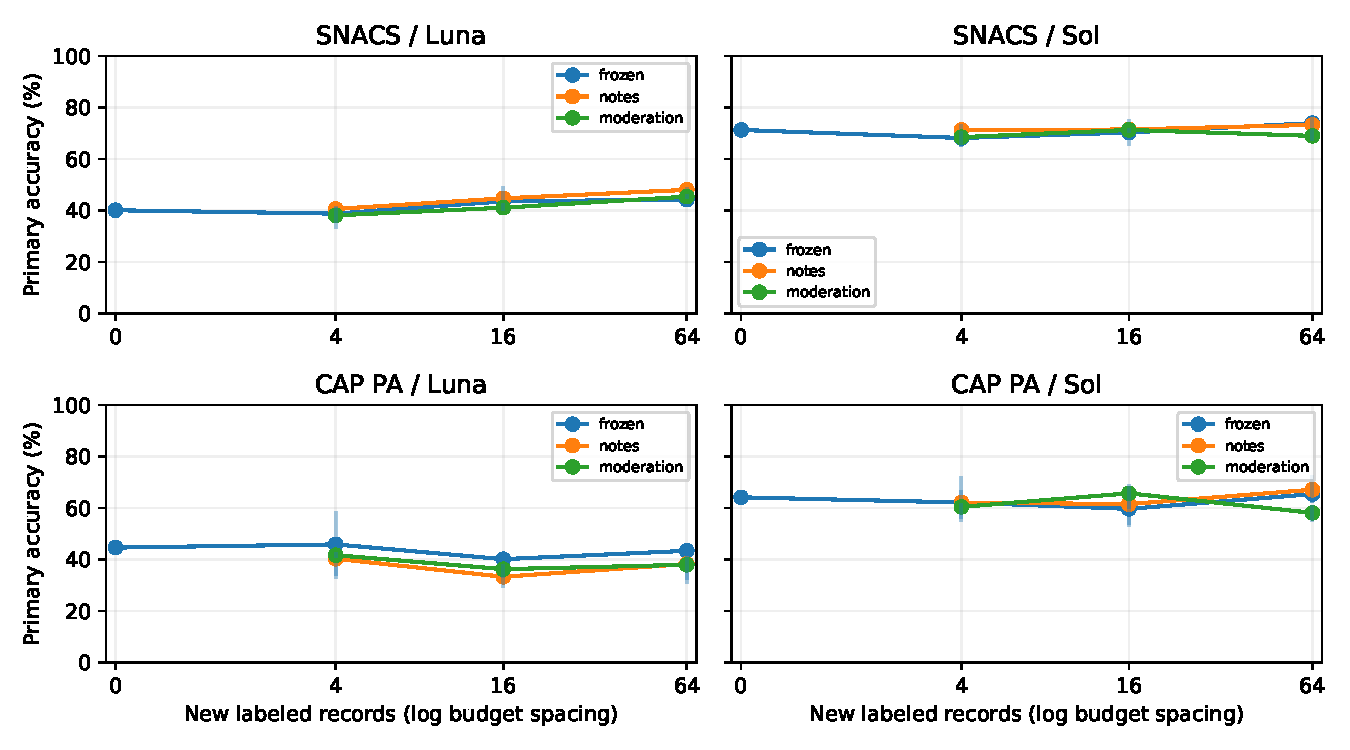
\includegraphics[width=.92\textwidth]{subscription-curves.pdf}
\caption{Observed completed-cell means. Vertical ranges span completed trajectory values, not confidence intervals; absent points are pending. The figure is descriptive until the planned trajectories complete.}
\end{figure*}


\subsection{Earlier Diagnostics Are a Separate Batch}
Before the subscription study, real dated GPT-5.4 API pilots ran on 24 SNACS sentences (50 targets), two adaptation trajectories, and budgets 0/4/16. Mini completed 275 of 312 prediction episodes; the larger tier completed 206 of 312. Unequal HTTP failures and call exhaustion confound their score differences. A later exact replay returned \texttt{credit\_balance\_exhausted}; the original logs do not justify labeling all earlier failures as quota exhaustion. These results remain archived and are not pooled with the new models or used as clean capability rankings.

Neither earlier SNACS program-permission arm executed a program. A subsequent Codex development run also used a note instead of executing code. These are failed manipulations of executable adaptation, not evidence that learned programs help or fail. The Fashionpedia engineering pilot used 16 genuine training and 16 validation images, one fixed supplied region each; sparse attribute IDs and incomplete instructions required separate auditing. It cannot support a visual guideline-learning claim. The earlier diagnostic paper and raw local traces are retained independently.

\section{Discussion}
Three boundaries must be distinguished. First, an agent may fail to retrieve a relevant rule or example even when it is authorized. Second, it may induce an incorrect rule or overgeneralize from a small sample. Third, the input may lack information needed to reproduce the published label. Total accuracy alone does not separate these causes. The exact-summary conflict audit addresses the third boundary under explicit assumptions; tool and asset logs diagnose parts of the first two, without expert adjudication replacing uncertainty.

Persistent assets also need a manipulation check. Writing a note, reading it, changing it at a larger budget, and improving held-out decisions are different events. Likewise, adaptation probes improving after a rewrite do not identify a stable benefit, because decoding may vary and the same data determine acceptance. A paired frozen-example control prevents the weaker comparison of a refined agent with a baseline denied the same examples, but does not remove compute differences.

The original question about unrestricted agents writing their own harness remains broader than this study. Allowing the evaluator or information permissions to change would undermine the comparison; allowing controlled executable assets is feasible, but meaningful program execution has not yet been established here. Future work needs a verified program intervention, expert-defined convention changes, stronger context-matched controls, and human sample-efficiency measurements. None is silently claimed as a completed result.

\section{Limitations}
This is a reviewable research sample, not a declaration of ACL submission readiness. Public benchmarks can be present in pretraining. We do not establish an expert-confirmed missing guideline rule or an audited unseen-construction split. The political task has sparse classes, historical guideline-alignment uncertainty, and unverified summary sufficiency. Approximate near-duplicate retrieval can miss related texts, while connected components can overmerge. The supplied-span linguistic track removes target discovery. The current two tasks are both textual; the visual pilot does not supply equivalent full-guideline evidence.

Model aliases, CLI overhead, tool-call caps, stochastic decoding, and subscription availability limit reproducibility and generalization. The two tiers differ in more than a known parameter count. Moderation is an adapted addendum workflow, not a faithful closest-paper numerical replication; its probe context and compute differ from ordinary retrieval. Three adaptation seeds do not establish a universal few-shot law. Stronger full-context controls, expert error adjudication, and prospective power analysis remain necessary for strong causal or sample-sufficiency claims.

\section*{Ethics and Reproducibility}
Original sources, material hashes, split IDs, predictions, purchase ledgers, settings, and failures are recorded. Raw corpora, images, full manuals, and source-bearing traces are not redistributed by default. CAP project-coded variables use CC BY-NC-SA 4.0; underlying source rights remain distinct. Credentials are neither extracted nor published. Political labels are project conventions, not universal definitions of meaning. Three AI reviewer agents critique resources, validity, and contribution; they are not human expert annotators or actual conference reviewers. AI assistance in research design, software, and writing is disclosed. Future human evaluation requires consent, appropriate compensation, and applicable review.
\bibliography{references}
\end{document}
